
\subsection{Introduction}

The history of neural network (NN) models have gone 
through several waves of popularity. The first 
one starts with the introduction of the perceptron
by \parencite{rosenblatt1958perceptron} and its training algorithm 
for classification in linearly separable problems.
Limitations brought up by 
\parencite{minsky} somehow reduced the enthusiasm
about these models by the early 70's.
The next period of success coincides with the emergence
of results presenting NNs as universal
approximators, e.g.\ \parencite{cybenko1989approximation}. Yet 
technical issues and the emergence of other paradigms like 
support vector machines led, essentially,
to a new stalmate by the early 2000's. Finally, several of the 
technical issues were solved, coinciding with the 
availability of faster computational tools,
improved algorithms and the emergence of
large annotated datasets. These produced outstanding 
applied developments leading, over the last decade, to the current boom 
surrounding deep NNs \parencite{10.5555/3086952}. 

This section overviews  
recent advances in NNs. 
There are numerous reviews with various emphasis 
including physical \parencite{cirac}, computational \parencite{chollet}, mathematical \parencite{maths} and pedagogical \parencite{teach} pùrposes, 
notwithstanding  those concerning different  application areas, 
from autonomous driving systems (ADS) \parencite{rumanos} to
drug design \parencite{hessler}, to name but a few. 
Our emphasis is on statistical
aspects and, more specifically, on Bayesian approaches
to NN models for reasons that will become 
apparent during the presentation but include mainly:
the provision of improved uncertainty estimates, which is
of special relevance in decision support under uncertainty; their 
increased generalization capabilities; their 
enhanced robustness against adversarial attacks; 
their improved capabilities for model calibration;
and the possibility of using sparsity-inducing priors
to promote simpler NN architectures.

We first recall basic results from (the now-called) 
shallow NNs.
Section \ref{sec:dnn_examples} then covers deep NNs, including their most
relevant 
variants, as well as classical and Bayesian approaches
for their analysis. Next, Section \ref{sec:dnn_examples}
presents two examples illustrating
diverse NN architectures. Finally, we present 
further topics referring to security, explainability and
interpretability and transfer 
learning of NNs and end up with a discussion.

%%%%%%%%%%%%%%%%%%%%%%%%%%%%%%%%%%%%%%%%%
\subsection{Shallow neural networks}
This section briefly introduces key concepts
about shallow networks to support later discussions on current approaches.
Our focus will be mainly on nonlinear regression 
problems. Specifically, we aim at approximating 
an $r$-variate response (output) $y$ with respect to $p$ explanatory 
(input) variables $x=(x_1,\ldots,x_p)$ through the 
model
\begin{eqnarray}\label{kantora}
  y         & = & \sum_{j=1}^m \beta_j \psi(x' \gamma_j) +
                    \epsilon %_i,~~i=1,\ldots,n
                    \nonumber\\
              & & \epsilon \sim N(0,\sigma^2),
                  \nonumber \\
              & & \psi(\eta) = \exp(\eta)/(1+\exp(\eta)).
                  \end{eqnarray}
This defines a neural network with one hidden 
layer with $m$ hidden neurons and logistic 
activation functions.
Figure \ref{figuradkk1} sketches 
a graphical model of a shallow NN with 10 inputs, 4 hidden nodes and 
2 outputs. 
\begin{figure}
    \centering
    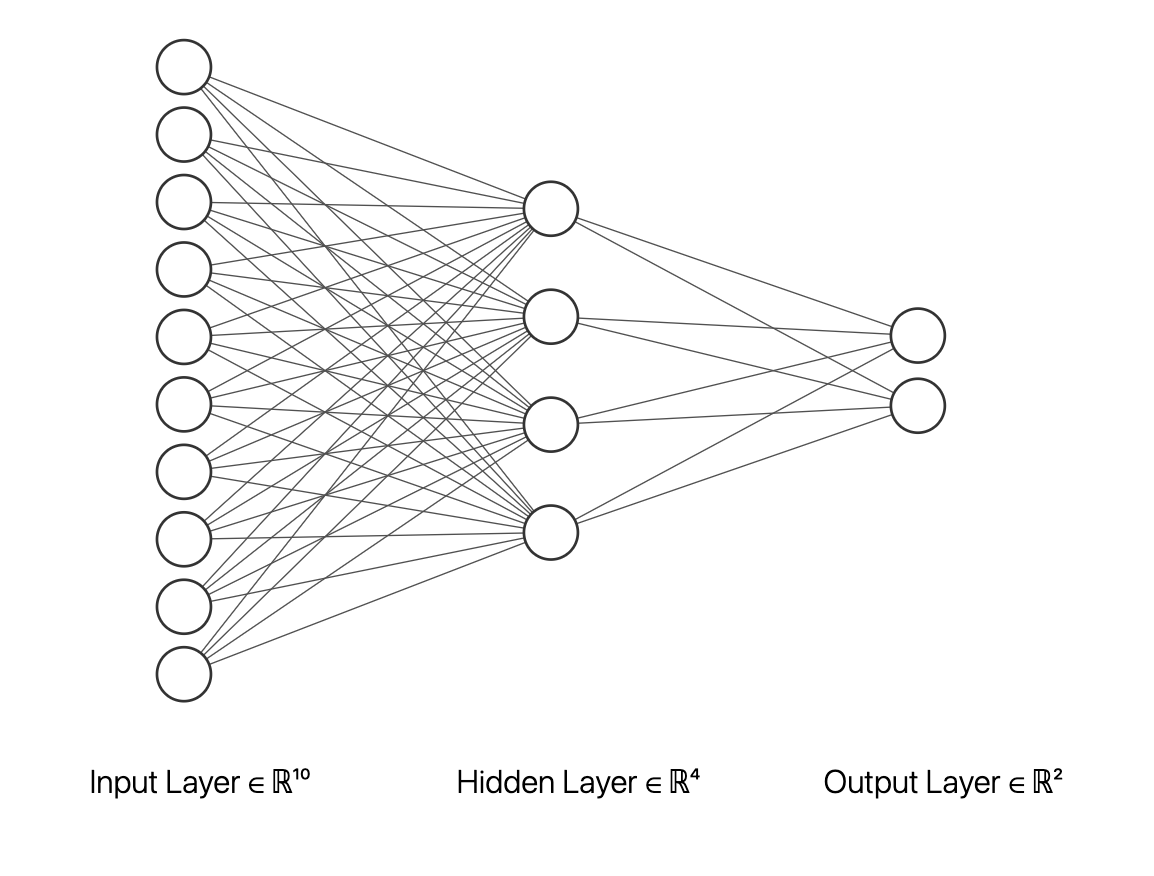
\includegraphics[scale=0.5]{figures/net1.png}
    \caption{A shallow NN architecture with 4 hidden nodes and 2 scalar outputs}
    \label{figuradkk1}
\end{figure}

Let us designate with $\beta=(\beta_1,\ldots,\beta_m)$ and $\gamma=(\gamma_1,\ldots,\gamma_m)$ the network parameters. $\sigma$  
will be considered a hyperparameter. Clearly, the model
is linear in $\beta$ but non-linear in  
$\gamma$. Interest in this type of models stems from 
results such as those of \parencite{cybenko1989approximation}
who presents them as universal approximators,
in the sense that any continuous function in the 
$r$-dimensional unit cube 
may be approximated by models of type
$\sum_{j=1}^m \beta_j \psi(x' \gamma_j)$
when the $\psi$
functions are sigmoidal (as with the logistic) and
$m\rightarrow \infty$. Our discussion focuses on $r=1$.



%%%%%%%%%%%%%%%%%%%%%%%%%%%%%%%%%%%%%%%
\paragraph{Classical approaches.}\label{sanchez}

Given $n$ observations $D=\{ (x_i, y_i), i=1,...,n \}$,
 maximum likelihood estimation (MLE) 
 computes the log-likelihood and maximises it 
leading to the classical non-linear least squares problem
\begin{equation}\label{pdt}
 \min_{\beta , \gamma } f (\beta , \gamma) = \sum _{i=1}^n f_i(\beta, \gamma)  =\sum _{i=1}^n \left( y_i -
  \sum_{j=1}^m \beta_j \psi(x_i'\gamma_j) \right)^2 
 \end{equation}

\noindent Quite early, researchers paid attention to the introduction of regularisers, such as weight decay $\ell_2$ penalization \parencite{krogh1992simple}, so as to improve model 
generalization, leading to the modified optimisation problem
\begin{equation}\label{kkdbak}
 \min  g(\beta ,\gamma) = f (\beta ,\gamma ) +
 h (\beta ,\gamma ), \end{equation}
where $h(\beta , \gamma )$ represents the regularisation 
term. For example, in the above mentioned case, the 
additional term is  
$h(\beta , \gamma )= \lambda _1 \sum \beta_i ^2 +
\lambda _2 \sum \sum \gamma _{ji} ^2$. 

Typically problems (\ref{pdt}) and (\ref{kkdbak}) are solved via steepest gradient descent \parencite{meza} through iterations of the type
\[
   (\beta, \gamma )_{k+1}=
   (\beta, \gamma )_{k}- \eta \nabla g (  (\beta, \gamma )_{k} ),
   \]
where $\eta $ is frequently chosen as a fixed small learning rate parameter and $\nabla g $ is the gradient of function $g$, with respect to 
$(\beta ,\gamma )$. 


\noindent    Very importantly,  the structure of the network and the 
    chain rule of calculus %take advantage of the 
    %above structure to 
    facilitates efficient estimation of the gradients 
    via backpropagation, e.g. \parencite{rumelhart1986learning}.
    
    A problem entailed by NN model estimation is the highly multimodal nature of
    the log-likelihood for three reasons:
    invariance with respect to arbitrary relabeling of
    parameters (these may
    be handled by means of order 
    constraints among the 
    parameters);
    that inherently due to non-linearity; and, finally, 
    node duplicity (which may be dealt 
    with a model reflecting uncertainty 
    about the number of nodes,
    as explained below).
A way to mitigate multimodality is to use a global optimization method, like multistart, but
this is very demanding computationally in this domain.

Finally, note that the same kind of NN models 
may be used for nonlinear auto-regressions in
time series analysis \parencite{menchero} and 
non-parametric 
regression \parencite{insuamuller}. Moreover,
similar models may be used for classification purposes,
although this 
 requires modifying the likelihood
\\parencite{bishop2006pattern} to e.g.\
\begin{equation}
    p(y | x, \beta, \gamma) = Mult(n=1, 
    p_1 (x, \beta, \gamma) , \ldots, p_K (x, \beta, \gamma) ),
\end{equation}
that is, a draw from a multinomial distribution with $K$ classes. 
Class probabilities
 can be computed using the softmax function,
$$
p_k = \frac{\exp{\beta_k \psi(x'\gamma_k)}}{\exp{\sum_{k=1}^K \beta_k \psi(x'\gamma_k)}}.
$$


%%%%%%%%%%%%%%%%%%%%%%%%%%%%%%%%%
\paragraph{Bayesian approaches.}\label{bayeshallow}
We discuss now Bayesian approaches to shallow NNs.
assuming standard priors 
in Bayesian hierarchical modeling, see e.g.\ \parencite{LavineWest}: 
$  \beta_i      \sim  N(\mu_\beta,\sigma_\beta^2)$
and 
  $\gamma_i     \sim  N(\mu_\gamma,S_\gamma^2)$,
  completed with priors over the hyperparameters
$\mu_\beta \sim N(a_\beta,A_\beta)$,
$\mu_\gamma \sim N(a_\gamma,A_\gamma)$,
$\sigma^{-2}_\beta \sim Gamma(c_b/2,c_bC_b/2)$,
$S_\gamma^{-1} \sim Wish(c_\gamma,(c_\gamma C_\gamma)^{-1})$ and
$\sigma^{-2} \sim Gamma(s/2, sS/2)$.
In this model, 
an informative prior probability model
is meaningful as parameters are interpretable. For example, the $\beta_ j$’s would reflect the
order of magnitude of the data $y_i$; typically positive and negative values for
$\beta _j$ would be equally likely, calling for a symmetric prior around 
0 with
a standard deviation reflecting the range of plausible values for $y_i$. Similarly,
a range of reasonable values for the logistic coefficients $\gamma_ j$ will be determined
%by the meaning of the data $y_i$ being modeled,
mainly to address smoothness
issues.

Initial attempts to perform Bayesian analysis
of NNs, adopted
arguments based on the asymptotic normality of the posterior, 
as in  
\parencite{mckay} and \parencite{buntineweigend}. However these methods
fail if they are dominated by  
less important modes. %; moreover, some of the 
%hypothesis underlying asymptotics are doubtful 
%in the NN context.
 \parencite{buntineweigend} mitigate this by finding several modes and
basing inference on weighted mixtures of the corresponding normal approximations, but we return to the same issue as some
important local modes might have been left out. An alternative view was argued
by \parencite{mckay}: inference from such schemes is 
 considered as approximate
posterior inference in a submodel defined by constraining the
parameters to a neighborhood of the particular local mode. Depending on
the emphasis of the analysis, this might be reasonable, especially if in a final
implementation our aim is to set the parameters at specific values,
the usual scenario in deep learning. We prefer
though to propagate the uncertainty in parameters, since this allows
better predictions, e.g. \parencite{raftery}. 

For this, an efficient 
Markov chain Monte Carlo (MCMC) scheme
may be used \parencite{muller1998issues}. It 
 samples from the posterior conditionals when available (steps 3, 9), and use
Metropolis steps (4-8), otherwise. To fight potential inefficiencies due to
multimodality, two features are built in 
 for
fast and effective mixing over local posterior modes:
whenever
possible, the $\gamma$ weights are 
partially marginalized; second,
these weights are resampled jointly.
The key observation is that,
given
 $\gamma $,
we actually have a standard hierarchical normal linear
model \parencite{french}. This facilitates sampling from the posterior marginals of the $\beta $ weights (step 3)
 and hyperparameters (step 9) and 
 allows marginalizing the model with respect
 to the $\beta$'s
  to obtain the marginal likelihood $p(D|\gamma, \nu)$
  (step 3), where $\nu=(\mu_\beta,\sigma_\beta,\mu_\gamma,S_\gamma,\sigma^2)$ designates the hyperparameters.
The procedure runs like the described in Algorithm \ref{alg:mcmc}.

\iffalse
{\tt 
\begin{enumerate}
  \item  Start with arbitrary $(\beta , \gamma ,\nu )$.\\
    Until convergence, iterate through 2-4
  \item  Given current $(\gamma,\nu)$, draw  
    $\beta$ from  
    $p(\beta|\gamma,\nu,y)$ (a multivariate normal).
    \item  For $j=1,...,m$,
    marginalizing in $\beta$ and given $\nu$, draw $\gamma_j$ through: \\
    Generate a candidate $\tilde\gamma_j \sim g_j(\gamma_j)$. \\
    Compute 
    $
       a(\gamma_j,\tilde\gamma_j) =
       \min\left(1,\frac{p(D |\tilde\gamma,\nu)}
                       {p(D |\gamma,\nu)}\right)
    $
    with $\tilde\gamma = (\gamma_1,\gamma_2,\ldots,\tilde\gamma_i, ...,\gamma_m)$.\\
    With probability $a(\gamma_j,\tilde\gamma_j)$ replace $\gamma_j$
    by $\tilde\gamma_j$. If not, preserve $\gamma_j$.
      \item Given $\beta$ and $\gamma$, replace $\nu$
        based on their posterior conditionals:\\
 $p(\mu_\beta|\beta,\sigma_\beta)$ is normal;
 $p(\mu_\gamma|\gamma,S_\gamma)$, multivariate normal;
 $p(\sigma_\beta^{-2}|\beta,\mu_\beta)$, Gamma; 
    $p(S_\gamma^{-1}|\gamma,\mu_\gamma)$, Wishart; 
    $p(\sigma^{-2}|\beta,\gamma,y)$, Gamma.
    \end{enumerate}
}
\fi

\begin{algorithm}[!ht]
\begin{algorithmic}[1]
\State Start with arbitrary $(\beta , \gamma ,\nu )$.
\While{not convergence} 
 \State Given current $(\gamma,\nu)$, draw  
    $\beta$ from  
    $p(\beta|\gamma,\nu,y)$ (a multivariate normal).
    \For{$j=1,...,m$, marginalizing in $\beta$ and given $\nu$ } 
    \State Generate a candidate $\tilde\gamma_j \sim g_j(\gamma_j)$.
    \State Compute 
    $
       a(\gamma_j,\tilde\gamma_j) =
       \min\left(1,\frac{p(D |\tilde\gamma,\nu)}
                       {p(D |\gamma,\nu)}\right)
    $
    with $\tilde\gamma = (\gamma_1,\gamma_2,\ldots,\tilde\gamma_i, ...,\gamma_m)$.
    \State With probability $a(\gamma_j,\tilde\gamma_j)$ replace $\gamma_j$
    by $\tilde\gamma_j$. If not, preserve $\gamma_j$.
    \EndFor
    \State Given $\beta$ and $\gamma$, replace $\nu$
        based on their posterior conditionals:
 $p(\mu_\beta|\beta,\sigma_\beta)$ is normal;
 $p(\mu_\gamma|\gamma,S_\gamma)$, multivariate normal;
 $p(\sigma_\beta^{-2}|\beta,\mu_\beta)$, Gamma; 
    $p(S_\gamma^{-1}|\gamma,\mu_\gamma)$, Wishart; 
    $p(\sigma^{-2}|\beta,\gamma,y)$, Gamma.
    
\EndWhile
\end{algorithmic}
 \caption{MCMC sampler}\label{alg:mcmc}
\end{algorithm}



\noindent For proposal generation distributions $g_j(\cdot)$,
normal multivariate distributions
$N(\gamma_j,c^2 C_\gamma)$ are 
adopted. % with $c=0.1$ work in
%applications. 
Appropriate values for $c$ can be found by trying
a few alternative choices until acceptance rates around
 0.25 are achieved \parencite{gamerman}. 

Combined with model augmentation to a variable architecture,
 this leads to a useful scheme
for complete shallow NN analyses as it allows for 
the identification of
architectures supported by data, by  
contemplating $m$ as an additional parameter.
A random $m$ with a prior 
favoring smaller values reduces posterior multimodality.
Moreover, as marginalization over $\gamma_ j$ requires inversion of matrices
of dimension related to $m$, 
avoiding unnecessarily large
hidden layers is critical to
mitigating computational effort.
 Thus, we assume 
a maximum size $m^*$ for the network and introduce 
indicators  $d_j$ suggesting whether node
$j$ is included ($d_j=1$) or not ($d_j=0$). 
We  also 
include a linear regression term $x'a$
to favor parsimony. On the whole, the model
becomes 
\begin{eqnarray*}
  y          & = & x_i'a + \sum_{j=1}^{m^*} d_j\beta_j \psi(x '\gamma_j) +
                    \epsilon \\ %_i,i=1,...,N\nonumber\\
                    & & \epsilon \sim N(0,\sigma^2),\nonumber \\
                    & &    \psi(\eta) = \exp(\eta)/(1+\exp(\eta)),
                        \nonumber \\
  Pr(d_j=0|d_{j-1}=1)   & = & 1-\alpha, \nonumber\\
  Pr(d_j=1|d_{j-1}=1)   & = & \alpha, \nonumber\\
  \beta_i    \sim  N(\mu_b,\sigma_\beta^2),& 
  a     \sim  N(\mu_a,\sigma_a^2), &   \gamma_i   \sim  N(\mu_\gamma,\Sigma_\gamma).
                \label{eq:model-var}
\end{eqnarray*}
Learning is done through a reversible jump sampler
\parencite{green} embedding our first algorithm.
As a consequence, we perform inference
about the architecture based on the distribution of 
 $p(m|D)$. 

 \parencite{neal2012bayesian} proposes using an 
algorithm merging conventional Metropolis-Hastings chains with sampling
techniques based on dynamic simulation, the currently popular
Hamiltonian Monte Carlo (HMC) approaches.
Let us designate by $\theta$ the NN 
weights, $\theta = (\beta, \gamma)$, and denote the potential energy function as
$$
U(\theta) = \tau_{\beta}\sum_{i=1}^m \beta_i^2/2 + \tau_{\gamma} \sum_{i=1}^m \gamma_i^2/2 + \tau \sum_{j=1}^n (y_j - f(x_i, \theta_i))^2/2,
$$
where $\tau_{\beta}, \tau_{\gamma}, \tau$ are hyperparameters 
controlling regularization, similarly to (\ref{kkdbak}). 
Let us also introduce the hamiltonian 
$$
H(\theta, r) = U(\theta) + \frac{1}{2} \sum_{i=1}^m r_i^2,
$$
with momentum variables $r$ of the same dimension as $\theta$; such 
 variables serve to accelerate the walk towards posterior modes. Then, the HMC scheme would be as described in Algorithm \ref{alg:hmc}.

\iffalse
{\tt 
\begin{enumerate}
  \item  Start with arbitrary $\theta_0 = (\beta _0, \gamma _0)$.\\
    Until convergence, iterate through 2-4
  \item  Given current $\theta_t$ and $r_t \sim \mathcal{N}(0, I)$, perform $T$ leapfrog integration
  steps 
  \begin{align*}
  r_{t + \frac{\epsilon}{2}} &= r_t - \frac{\epsilon}{2}\nabla U(\theta_t) \\
   \theta_{t+ \epsilon} &= \theta_t + \epsilon  r_{t + \frac{\epsilon}{2}} \\
   r_{t + \epsilon} &= r_{t + \frac{\epsilon}{2}} - \frac{\epsilon}{2}\nabla U(\theta_{t+ \epsilon})
    \end{align*}
    to reach  $\theta^*$ and $r^*$. % be the final solution 
    %and its corresponding momentum.
\item Compute $\alpha(\theta_t, \theta^*) = \min \left\{ 1, \frac{\exp H(\theta^*, r^*)}{\exp H(\theta_0, r_0)} \right\} $
\item Accept $\theta^*$ with probability $\alpha(\theta_t, \theta^*)$, else discard it.
    \end{enumerate}
}
\fi


\begin{algorithm}[!ht]
\begin{algorithmic}[1]
\State Start with arbitrary $\theta_0 = (\beta _0, \gamma _0)$.
\While{not convergence}
  \State Given current $\theta_t$ and $r_t \sim \mathcal{N}(0, I)$, perform one or more leapfrog integration
  steps 
  \begin{align*}
  r_{t + \frac{1}{2}} &= r_t - \frac{\epsilon}{2}\nabla U(\theta_t) \\
   \theta_{t+ 1} &= \theta_t + \epsilon  r_{t + \frac{1}{2}} \\
   r_{t + 1} &= r_{t + \frac{1}{2}} - \frac{\epsilon}{2}\nabla U(\theta_{t+ 1})
    \end{align*}
    to reach  $\theta^*$ and $r^*$.
    \State Compute $\alpha(\theta_t, \theta^*) = \min \left\{ 1, \frac{\exp H(\theta^*, r^*)}{\exp H(\theta_t, r_t)} \right\} $.
   \State Accept $\theta^*$ as $\theta_{t+1}$ with probability $\alpha(\theta_t, \theta^*)$, else discard it. 
  
 \EndWhile
 \end{algorithmic}
 \caption{HMC sampler}\label{alg:hmc}
\end{algorithm}





%%%%%%%%%%%%%%%%%%%%%%%%%%%%%%%%%%%%%%%%
\subsection{Deep neural networks}\label{sec:dnn_examples}

Training by backpropagation has been in use 
for many years by now.
The decade of the 2010's saw major developments
leading to 
the boom around deep learning \parencite{10.5555/3086952}
or inference and prediction with deep NNs. 
Such advances include:
the availability of fast GPU kernels and routines
facilitating much faster training;
the access to massive amounts of data (e.g.\ Imagenet), which prevented overfitting to smaller datasets; 
the creation of new architectures, which prevented  convergence issues, such as the vanishing gradient problem; 
and, finally, the provision of automatic differentiation libraries such as Keras, Caffe or Theano.
Figure \ref{figuradkk} displays a description
of what are now designated 
deep NNs, that is NNs with more than one hidden
layer, four in the portrayed case.
\begin{figure}
    \centering
    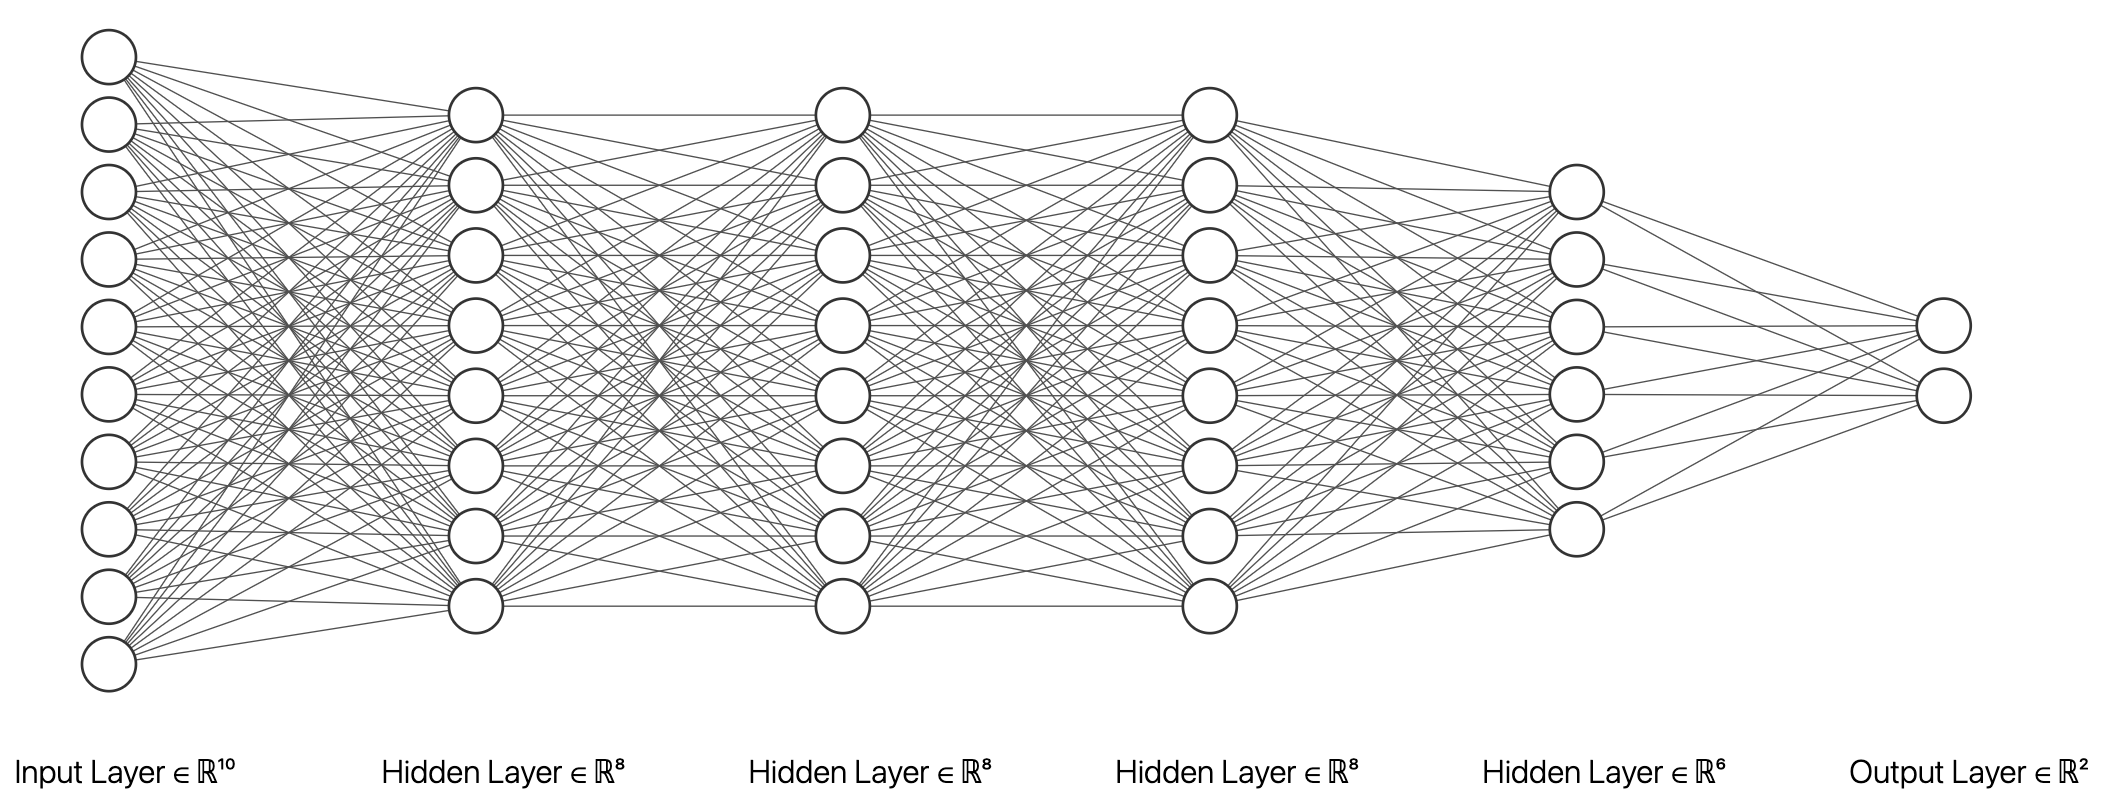
\includegraphics[scale=0.35]{figures/net2.png}
    \caption{A deep NN architecture with four hidden layers and 2 scalar outputs}
    \label{figuradkk}
\end{figure}


A deep NN may be defined through   
a sequence of functions $\lbrace f_0, f_1, ..., f_{L-1} \rbrace$, each parametrized by some weights $\gamma_l$
of dimension $m_l$  (the corresponding number of hidden nodes) and the output of each layer being the input of the following one, as in
$$
    z_{l+1} = f_l ( z_l, \gamma_l).
$$
Lastly, we compute a prediction from the hidden activations of the last layer, as before:
\begin{eqnarray}
y         & = & \sum_{j=1}^{m_L} \beta_j z_{L,j} +
                    \epsilon %_i,~~i=1,\ldots,n
                    \nonumber\\
              & & \epsilon \sim N(0,\sigma^2),
                  \nonumber \\
\end{eqnarray}

Modern architectures do not longer require the
$f_l$ functions to be sigmoidal (like the  
logistic functions in (\ref{kantora})) and include  
the rectified linear unit (ReLU), the leaky ReLU
or the exponential LU. In particular, these functions mitigate the vanishing gradient problem \parencite{kolen2001gradient} that 
plagued earlier attempts with deep architectures using sigmoidal
activation functions: the derivative of the logistic function is $\psi(z)' = \psi(z)(1 - \psi(z))$, with $\psi(z) = \frac{1}{1 + e^{-z}}$ and since the output of the logistic function is bounded in $\left[ 0, 1 \right]$, a concatenation of layers using this activation function makes the gradient quickly vanish to zero due to the chain rule. Alternative activation functions, such as the ReLU \parencite{glorot2010understanding}, seem to alleviate this problem, in addition to having other benefits such as being faster to compute both the activation and its derivative.

%%%%%%%%%%%%%%%%%%%%%%%%
%\subsubsection{Variants} 
Beyond the above generic deep architectures 
a few important specialised models have emerged which 
are relevant in specific application domains,
as we describe now. 
%%%%%%%%%%%%
\paragraph{Convolutional neural networks} 
CNNs are typically used 
 in computer vision tasks and related signal processing applications.
 Stemming from the work by Le Cun and coauthors  
  \parencite{lecun89, lecun98} and their original 
  LeNet5 design, they achieved major
 successes  in  competitions \parencite{NIPS2012_c399862d}
 leading to architectures like 
 AlexNet       \parencite{NIPS2012_c399862d}, VGGNet \parencite{simonyan2014very} or
 GoogleNet \parencite{szegedy2015going}, reaching 
 superhuman performance in 
 image recognition tasks.
 
 In CNNs, the layer transformation is taken to be a convolution with some 2D or 3D kernel; this makes the network able to recognise patterns independently of their location or scale in the input, a desirable property in computer vision tasks known as spatial equivariance. In addition, by replacing a fully-connected layer with a small kernel (typically, in the 2D case these are of shapes $3\times3, 5\times 5$ or $7\times 7$), there is weight sharing amongst the unit from the previous layer and this allows reducing 
 the number of parameters and prevents overfitting.
 Thus, the typical convolutional network layer is composed of several sub-layers:
 \begin{itemize}
     \item A convolution operation, as before, 
     serving as an affine transformation of the representation from the previous layer. A layer can apply several convolutions in parallel to produce a set of linear activations.
     \item A non-linear layer, such as the rectifier (based on the ReLU function), converting the previous activations to nonlinear ones.
     \item An optional pooling layer, which replaces the output of the net at a certain position with a summary statistic of 
     the nearby outputs (typically the mean or the maximum).  
 \end{itemize}
 
 The use of the convolution may be viewed as introducing an infinitely strong prior probability distribution over the parameters of a linear layer, in the sense that the prior places zero probability mass over certain parameters, imposing that the weights for one hidden unit must be identical to the weights of its neighbor, yet shifted in space. In a 
  similar spirit, pooling can be regarded as placing an infinitely strong prior about the function having to be invariant to small translations. If this assumption is also held in the dataset, it can vastly improve the statistical efficiency of the network.
 
Current advances in CNNs pursue model scaling, suggesting that carefully balancing network depth, width, and resolution can lead to improved performance,
as with ResNets \parencite{he2016deep} or EfficientNets \parencite{tan2019efficientnet}.



%%%%%%%%%%%%
\paragraph{Recurrent neural networks} RNNs are typically used for sequence processing, as in natural language processing (NLP), e.g.\ \parencite{hochreiter1997long} and \parencite{chung2014empirical}. They have feedback connections which make the network aware of temporal dependencies in the input.

Let $x_t$ denote the $t$-th token (usually a word, but could even be 
a smaller part) in the input sequence. A simple recurrent layer can be described as
$$
h_t = \psi(W_x x_t + W_h h_{t-1} + b_h)
$$
with the output at that time-step given by
$$
y_t = \psi(W_y h_t + b_y),
$$
where $\psi$ is a non-linear activation function, such as the logistic or the hyperbolic tangent functions. This is the Elman network \parencite{cruse2006neural}. Note that weights are shared between different time-steps. In a similar vein to the infinitely strong prior from CNNs, this parameter sharing allows the network searching for patterns independently of their position in the sequence, yet also taking into account information from previous positions thanks to its feedback loop.

For training purposes, all of the previous loops must be unrolled back in time, and then perform the usual gradient descent routine.
This is called \emph{backpropagation through time} \parencite{58337}.
Backpropagating through long sequences may lead to problems
of either vanishing or exploding gradients. Thus, 
simple architectures like Elman's cannot be applied to long inputs, as those arising in NLP. 
As a consequence, gating architectures which improve the stability have been proposed, and successfully applied in real-life tasks,
such as long 
short-term memory (LSTM) \parencite{hochreiter1997long} and gated recurrent unit (GRU) networks \parencite{cho2014learning}. 
External memory-augmented RNNs have also been proposed to tackle symbolic reasoning tasks, such as the neural Turing machine \parencite{graves2014neural} or the differentiable neural computer \parencite{graves2016hybrid}.
From a statistical point of view, RNNs describe directed graphical models similar to those of hidden Markov models (HMMs), but more efficiently parameterized. A fruitful line of research aims to bridge the gap between classical Markov models and neural parameterizations, as in deep Kalman filters \parencite{krishnan2015deep} or deep Markov models \parencite{krishnan2016structured}.
%Assuming that each (discrete) token in the input can take $k$ different values, a HMM for sequences of length $T$ requires $\mathcal{O}(k^T)$ parameters to represent
%the joint distribution over the sequence; in turn, RNNs keep this requirement constant, independently of the length of the input, thanks to parameter sharing.  In the realm of memory-augmented RNNs, special attention should be given to the Kanerva machine \parencite{wu2018kanerva}, a generative distributed memory updated in a Bayesian fashion.



%%%%%%%%%%%%
\paragraph{Transformers} These architectures substitute the sequential processing from RNNs by a more efficient, parallel approach inspired by 
attention mechanisms \parencite{vaswani2017attention,bahdanau2014neural}. Their basic building components are scaled dot-product attention layers:
let $x_i$ be the embedding\footnote{An embedding layer is a linear layer that projects a one-hot representation of words into a lower-dimensional space.} of the $i$-th token in an input sequence;
this is multiplied by three weight matrices to obtain: 1) a query vector, $q_i = W_q x_i$; 2), 
 a key vector $k_i = W_k x_i$;
 and, 3) a value vector, $v_i = W_v x_i$. The output of the attention layer is computed, parallelizing along the input position $i$, 
 through 
$$
\mbox{softmax}\left(\frac{q k^{'}}{\sqrt{d_k}}\right) v,
$$
 a weighted average of the components of the value vector, where the average is 
computed as a normalized dot product between the key and query vectors. Thus, the attention layer produces activations for every token  that contains information not only about the token itself, but also a combination of other relevant tokens weighted by the attention weights.

Each layer of a transformer model usually comprises several 
parallel layers, enabling the net to pay attention to different parts of the input simultaneously. Attention layers are alternated with  feed-forward layers in what is designated an encoder block. These 
 can be stacked until the final layer, outputting the probabilities for classification tasks. If the task requires producing outputs that are variable in length, as in automatic translation or summarization, decoder layers must be used, which replicate the work of encoders until output generation, in a similar spirit to the seq2seq models initiated a few years before with recurrent architectures \parencite{sutskever2014sequence}.

Since transformer-based models are more amenable to parallelization,
 they have been trained over massive datasets in the NLP domain, leading to architectures such as Bidirectional 
Encoder Representations for Transformers (BERT) \parencite{devlin2018bert}
or the series of Generative
pre-trained Transformer (GPT) models \parencite{radford2018improving, radford2019language, brown2020language}. Current research avenues aim to scale such models to increasingly longer sequences \parencite{tay2020long} or studying the societal and environmental issues of training gargantuan-scale models over potentially biased textual data \parencite{bender2021dangers}.
%From a Bayesian point of view, recent evidence suggests that transformers may be viewed as maximum  a posteriori (MAP) estimators in  Gaussian mixture models \parencite{movellan2020probabilistic}. %Further research is necessary in this direction, since we hypothesize that the Bayesian framing may help in searching for more efficient attention kernels or the adoption of sparsity-inducing priors, which could help in keeping the size of the larger architectures under control.


%%%%%%%%%%%%%
\paragraph{Generative models} 
The models from the previous paragraph belong to the discriminative family of models. Discriminative models directly learn the conditional distribution $p(y|x)$ from the data.
Generative models, as opposed to discriminative ones, take a training set, consisting of samples from a distribution $p_{data}(x)$, and learn to represent an estimation of that distribution, resulting in another probability distribution, $p_{model}(x)$. Then, one could fit a distribution to the data by performing MLE,
$$
\max_{\theta} \sum_{i=1}^n \log p_{model} (x_i | \theta),
$$
or MAP estimation if a prior over the parameters $\theta$ is also placed. Fully visible belief networks \parencite{10.5555/2998828.2998922} are a class of models that can be optimized this way. They are computationally tractable since they decompose the probability of any given $d-$dimensional input as $p(x | \theta) = \prod_{i=1}^d p(x_i | x_1 , \ldots x_{i-1}, \theta)$. Current architectures that fall into this category include WaveNet \parencite{oord2016wavenet} and pixel recurrent neural networks \parencite{pmlr-v48-oord16}. Normalizing flows can also make the distribution more flexible by means of stacking a series of suitably computable transformations \parencite{rezende2015variational}.
Another important family of models are called autoencoders \parencite{autoencoders,kingma2013auto}. They perform dimensionality reduction 
using a sequence of non-linear transformations.

%%%%%%%%%%%%%
\paragraph{Generative adversarial networks} GANS  perform density estimation in high-dimensional spaces formulating a game between two players, a generator and a discriminator \parencite{goodfellow2014generative}. They belong to the family of generative models; however, GANs do not explicitly model a distribution $p_{model}$, i.e., they cannot evaluate it, only generate samples from it.
GANs define a probabilistic graphical model containing observed variables $x$ (the input data, like an image or text) and latent variables $z$. Then, both players can be represented as two parameterized functions via NNs. Thus, the generator will be of the form $f_G(z, \theta_G)$, i.e., a NN that takes as input a latent vector and is parameterized through weights $\theta_G$. Note that the last layer will depend on the shape and range of the data $x$. Likewise, the discriminator will be a function $f_D(x, \theta_D)$ receiving a (fake or real) sample $x$ and outputting a probability for each of these two classes. Therefore, the final activation function will be 
the sigmoid function. Each network has its own objective function. For the discriminator, the cost is
$$
\mathcal{L}_G(\theta_D, \theta_G) = -\dfrac{1}{2} \mathbb{E}_{x \sim p_{data}} \log f_D(x, \theta_D) -\dfrac{1}{2} \mathbb{E}_z \log (1 - f_D(f_G(z, \theta_G), \theta_D)),
$$
that is, the standard cross-entropy for classifying real data as 1, and fake data from $G$ as 0. As for the generator objective, we could take $\mathcal{L}_D(\theta_D, \theta_G) = -\mathcal{L}_G(\theta_D, \theta_G)$,
and, consequently, both networks would play a minimax game.
Now, both players update their weights sequentially, typically using SGD or any of its variants.
However, while being helpful for theoretical analysis, 
this minimax game entails a practical problem: when the discriminator successfully rejects fake samples from the generator, since the last network is using the opposite loss function, its gradient vanishes, making the generator unable to learn how to fool the discriminator and produce better quality samples.
The vast literature on GANs is usually devoted to the previous problem, such as approaches based  on optimal transport, by minimising a Wasserstein distance between fake generated data and real data examples \parencite{arjovsky2017wasserstein}. In \parencite{nowozin2016f}, GANs are trained using variational divergence minimization, with the possibility of choosing any $f$-divergence \parencite{CIT-004}.

%One approach is via heuristics. For instance, by flipping the labels for the generator, we can use as objective function
%$$
%\mathcal{L}_D(\theta_D, \theta_G) = -\dfrac{1}{2} \mathbb{E}_{x} \log f_D(f_G(z, \theta_G), \theta_D).
%$$


%While GANs have already produced astonishing results in areas such as image generation \parencite{Karras2019stylegan2,brock2018large}, they are still pervaded by problems such as training instabilities or mode collapse, in which the generator gets stuck on a mode and the samples generated thus lack diversity. A probabilistic approach to deal with this problem was introduced in \parencite{dieng2019prescribed}, using a regularizer based on the entropy. We expect that the adoption of Bayesian methods,
% such as efficient SG-MCMC samplers (Section 3.3.1), will be helpful
%in improving the diversity of samples generated by GANs.

%%%%%%%%%%%%%%%%%%%%%%%%%%%%%%%%%%%%%%
\paragraph{Classical approaches.}

In principle, we could think of using 
with deep NNs the approach in Section \ref{sanchez}. However,
 large scale problems bring in two major
computational issues: first, the 
evaluation of the gradient of the loss wrt the parameters
requires going through all observations
 becoming too expensive when $n$ is large;
second, estimation of the gradient component
for each point requires a much longer backpropagation recursion through the various levels of the
deep network, 
entailing again a very high computational 
expense. 

Fortunately, these computational demands are mitigated
through the use of classical stochastic gradient descent
(SGD)
methods \parencite{robbins}
to perform the estimation \parencite{bottou2010large}. SGD is the current workhorse of large-scale optimization and 
allows training deep NNs over large datasets by mini-batching: rather than going through the whole batch at each stage, just pick a small sample
(mini batch) of observations and do the corresponding
gradient estimation by backpropagation. This is reflected in the Algorithm \ref{alg:sgd}, which departs from an
initial $\theta$.

\iffalse
{\tt 
\begin{enumerate}
  \item  While stopping criterion not met, do
  \begin{enumerate}
      \item  Sample a size $l$ minibatch 
      $((x^{(1)}, y^{(1)}),..., (x^{l},y^{l})) $
              from training set 
            \item Compute a gradient estimate
      $g_k = \frac{1}{l} \sum_{i=1}^l \nabla_{\theta} f_i(\theta_k) + \nabla_{\theta} h(\theta_k)$
      \item Update $\theta_{k+1} $ = $\theta_k -\epsilon _k g_k$
      \item $k=k+1$
      \end{enumerate}
          \end{enumerate}
}
\fi

\begin{algorithm}[!ht]
\begin{algorithmic}[1]
\While{stopping criterion not met}
  \State Sample a size $l$ minibatch 
      $((x^{(1)}, y^{(1)}),..., (x^{l},y^{l})) $
              from training set. 
\State Compute a gradient estimate
      $g_k = \frac{1}{l} \sum_{i=1}^l \nabla_{\theta} f_i(\theta_k) + \nabla_{\theta} h(\theta_k)$
\State    Update $\theta_{k+1} $ = $\theta_k -\epsilon _k g_k$ 
\State    $k=k+1$ 
 \EndWhile
\end{algorithmic}
 \caption{Stochastic gradient descent}\label{alg:sgd}
\end{algorithm}

\noindent The standard Robbins-Monro conditions require
that $\sum _k \epsilon_k = \infty$ and 
$\sum _k \epsilon _k^2 < \infty $ for convergence to the optimum.

Recent work has explored ways to 
speed up convergence towards the local optimum, 
leading to several SGD variants, including the 
 addition of a momentum, as in AdaGrad, Adadelta or Adam \parencite{kingma2014adam,duchi2011adaptive,zeiler2012adadelta}. The essence of these methods is to take into account not only a moving average of the gradients, but also an estimate of its variance, so as to dynamically adapt the learning rate. 

Let us finally mention 
several techniques to improve generalization and convergence of neural networks, such as dropout \parencite{srivastava2014dropout}, batch normalization \parencite{ioffe2015batch} or weight initialization \parencite{glorot2010understanding}.


%%%%%%%%%%%%%%%%%%%%%%%%%%%%%%%%%%%%

\subsection{Examples}\label{sec:nn_examples}
We illustrate learning with deep NNs with two examples portraying
different architectures and application domains. Code for the experiments was done using the \texttt{pytorch} library \parencite{paszke2017automatic} and is released at \url{https://github.com/vicgalle/nn-review}.

%%%%%
\paragraph{CNNs for image recognition.}\label{kkvision}

We describe an image classification task with a standard CNN, VGG-19, showcasing the superior performance when compared to non-convolutional and non-deep approaches in this application domain. As benchmark, we use the CIFAR-10 dataset \parencite{krizhevsky2014cifar},
which consists of 60000 32x32 colour images in 10 classes. As baselines, we use a linear multinomial regression model, and a three hidden layer MLP with 200 units each with ReLU activations.

All models are trained for 200 epochs\footnote{An epoch is defined as a pass over the full training dataset.} and minibatches of 128 samples, using SGD with learning rate of 0.1 and  momentum of 0.9.
The learning rate is adapted with the cosine annealing scheme in  \parencite{loshchilov2016sgdr}. We place Gaussian priors over all parameters (thus equivalent to $\ell_2$ regularization) and use SWA on top of the SGD optimizer, to make predictions using an ensemble of several particles, in a Bayesian way.

\begin{figure}[hbt]
\centering
  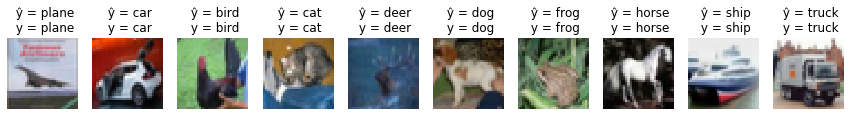
\includegraphics[width=1.\linewidth]{figures/cifar.png}
  \caption{Ten random samples from the CIFAR-10 dataset and their corresponding predictions and true labels using the VGG architecture.}
  \label{fig:cifar}
\end{figure}

Figure \ref{fig:cifar} presents ten random images from the test set
and Table \ref{tab:cnn} displays results. Notice how the linear model performs poorly with just test accuracy of 38\% , whereas increasing the flexibility of the models critically improves 
accuracy; a MLP performs slightly better.
However, by imposing strong priors about the dataset, such as translation equivariance thanks to the convolutional layers and pooling, state-of-the-art results are achieved.

\begin{table}[ht]
\caption{Results over the CIFAR-10 test set.}
\centering
\begin{tabular}{ll}
Model & Test acc. \\
\hline
Linear &  $38.10\%$ \\
MLP &  $50.03\%$\\
VGG-19 &  $93.29\%$ 
\end{tabular}
\label{tab:cnn}
\end{table}

%%%%%%%%%%%%%%%
\paragraph{Transformer and recurrent models for sentiment analysis.}
This is an example with text to undertake sentiment analysis, classifying movie reviews with architectures tailored to NLP tasks. As benchmark, we use the IMBD movie review dataset 
from \parencite{maas-EtAl:2011:ACL-HLT2011}, in which a review in raw text must be classified into one of two classes: positive or negative
sentiment. 

The recurrent model consists of a LSTM network with two layers, each with hidden dimension of 256 plus a dropout of 0.5 serving as a regularizer. We also consider a simple Transformer-based model, with two encoder layers, of hidden dimension 10 plus similar dropout. For both models, the input sequence is represented as a list of one-hot encoded vectors, representing the presence of a word from a vocabulary of the 5000 most common tokens. This representation is embedded into a space of 100 dimensions
(16 in the Transformer case) by means of an affine transformation, before applying architecture-specific layers. Both models are trained using the Adam optimizer with a constant learning rate of 0.001.
%The input sequence is represented as a list of one-hot encoded vectors, representing the presence of a word from a vocabulary of the most common 5000 tokens. This discrete representation is embedded into a space of 100 dimensions (16 dimensions in the Transformer case) by means of an affine transformation, before applying the architecture-specific layers. 
%Both models are trained using the Adam optimizer with a constant learning rate of 0.001.

We also consider a bigger, transformer-based model consisting of the recent RoBERTa architecture \parencite{liu2019roberta}, 
initially pretrained on a big corpus of unsupervised raw  English text, and then fine tuned for two epochs on the IMDB training set. %As we 
 %discuss in Section \ref{sec:transfer}, pretraining with data from different tasks or domains can crucially improve the performance of Transformers, since this helps in building better representations of written language.

Table \ref{tab:examples} shows two random examples from the IMDB dataset.
Results over the full test set are displayed in Table \ref{tab:nlp}. Notice how the Transformer-based models are superior to the recurrent baseline, and the extra benefits thanks to the usage of transfer learning.

{\footnotesize
\begin{table}[ht]
\caption{Four random review samples and their corresponding predictions and true labels from the RoBERTa model.}
\centering
\begin{tabularx}{\textwidth}{Xll}
Text input & Prediction & True label \\
\hline
 {\scriptsize \texttt{HOW MANY MOVIES ARE THERE GOING TO BE IN WHICH
AGAINST ALL ODDS, A RAGTAG TEAM BEATS THE BIG GUYS
WITH ALL THE MONEY?!!!!!!!! There's nothing new in
"The Big Green". If anything, you want them to
lose. Steve Guttenberg used to have such a good
resume ("The Boys from Brazil", "Police Academy",
"Cocoon"). Why, OH WHY, did he have to do these
sorts of movies during the 1990s and beyond?! So,
just avoid this movie. There are plenty of good
movies out there, so there's no reason to waste
your time and money on this junk. Obviously, the
"green" on their minds was money, because there's
no creativity here. At least in recent years,
Disney has produced some clever movies with Pixar.} } &   Negative & Negative   \\
\hline
 {\scriptsize \texttt{When I first heard that the subject matter for
Checking Out was a self orchestrated suicide
party, my first thought was how morbid, tasteless
and then a comedy on top of that. I was skeptical.
But I was dead wrong. I totally loved it. The
cast, the funny one liners and especially the
surprise ending. Suicide is a delicate issue, but
it was handled very well. Comical yes, but tender
where it needed to be. Checking Out also deals
with other common issues that I believe a lot of
families can relate with and it does with tact and
humor. I highly recommend Checking Out. A MUST
SEE. I look forward to its release to the public.} } &   Positive & Positive   \\

\end{tabularx}
\label{tab:examples}
\end{table}
}

\begin{table}[h]
\caption{Results over the IMDB test set.}
\centering
\begin{tabular}{ll}
Model & Test acc. \\
\hline
LSTM &  $81.99\%$ \\
Simple Transformer &  $87.49\%$ \\
RoBERTa &  $94.67\%$\\
\end{tabular}
\label{tab:nlp}
\end{table}











%%%%%%%%%%%%%%%%%%

\iffalse


\subsection{Other topics}
We conclude with a discussion of three transversal topics in NN
research and applications which are gaining much traction at the moment: how may we protect the predictions of deep
learning models from malicious attacks perturbing data; how can we interpret or explain the predictions of a deep model; and, finally, how may we reuse what a deep model
learns in a domain into another related context. 

%%%%%%%%%%%%%%%%%%%%%%%%%%%%%%


\subsubsection{Explainability}

Section \ref{bayeshallow} described how the parameters 
in shallow NNs remained interpretable and this  guided
prior assessment. Explainability and interpretability are also important aspects for deep learning models,
where a decision depends on an enormous amount of weights and parameters. Here, the parameters are often abstract and disconnected from the real world, which makes it difficult to interpret and explain their results.


Thus, when properly trained, predictions obtained by
NNs may have a high accuracy but humans
often perceive the models as black boxes, their insights
remaining mostly
opaque for humans. Particularly understanding 
the entailed decision making in highly sensitive
areas such as healthcare, criminal justice, defense or finance, is of paramount importance,
requiring it to be more transparent, accountable, and understandable
for humans.
At this point is worth mentioning how the 
EU General Data Protection Regulation (GDPR) could require AI providers to deliver explanations of results of automated decision-making based on their personal data, even leading to the prohibition of the use of opaque models that are used for certain applications.

There are various approaches to the problem as 
thoroughly reviewed in ****** (2020).
One possibility is to use interpretable models,
 easily comprehensible for humans,
as cogently argued by \parencite{rudin2019stop} who claims 
that in many contexts we may perform with such models 
almost as well as with deep models.
 While using interpretable models might be appropriate for some
  contexts, they come at the cost of flexibility, accuracy, and usability.
  Alternatively, sometimes an interpretable surrogate model of the black box model is generated to gain interpretability, either globally or locally around
some test input, as with LIME \parencite{ribeiro2016model} or SHAP \parencite{lundberg2017unified}.
Finally, there are attempts to create methods for explaining 
black box models with two main broad strategies: globally
extracting an explanation from a model that is representative for some specific
data set; and locally extracting an explanation for a single test input 
 and the corresponding prediction.
  \parencite{samek2017explainable} describe different methods for visualizing and explaining deep learning models like the Layer-wise relevance propagation (LRP). 
 
 
 %%%%%%%%%%%%%%%%%%%%%%%%%%%%%%%%%%%%%%%%%
\subsubsection{Transfer learning}\label{sec:transfer}

The training of huge neural models requires large amounts of labelled data, such as images, typically in the order of thousands to millions. In cases where human labelling of training data is not feasible 
for scaling to those magnitudes, it is possible to leverage similar datasets, even not for the same task. This is called transfer learning \parencite{tan2018survey,pan2009survey}, and fundamentally consists of taking a model previously trained over a massive dataset and then fine-tune the model in the final task, with a much smaller dataset. The adoption of pretrained models allows the practitioner to save in computational costs, because it significantly shortens the training time for the final dataset, and often leads to improved performance, thanks to the already learnt knowledge of the pretrained model. In addition, the quantity of labelled data can be drastically reduced by strategically choosing the data points to be annotated. Techniques developed to automatize this idea fall under the term of active learning, and the Bayesian approach offers a principled and sound framework for it, see e.g. \parencite{houlsby2011bayesian}.

Transfer learning has enjoyed extraordinary success in fields
such as computer vision and natural language processing. With image data \parencite{girshick2014rich,NIPS2014_375c7134}, it is common to pretrain a CNN on a huge dataset (typically Imagenet, \parencite{deng2009imagenet}, with over 1M images from 1000 categories) and then use the CNN either as an initialization (this can be regarded as specifying a Bayesian prior from the previous task) or as a feature extractor for the custom task. Typically, one removes the last layer of the pretrained CNN (that which projects the hidden representation to the 1000 logits for Imagenet), and places another linear layer with softmax activations for the task of interest, or takes the hidden representation to use with another classifier, such as a support vector machine or a random forest \parencite{sharif2014cnn}. The Deep Image Prior is also an interesting example as it shows that a randomly-initialized neural network can be used as a handcrafted prior with excellent results in standard inverse problems such as denoising, super-resolution, and inpainting \parencite{ulyanov2020deep}.

Transfer learning with textual data has gained traction more recently, with the advent of gargantuan-sized language models. Models such as BERT \parencite{devlin2018bert}, or the family of GPT models \parencite{radford2018improving,radford2019language,cc:BrownMannRyderSubbiahEtAl:2020:language-models}
have achieved the state-of-the-art in many NLP tasks. 
In this case, pretraining fundamentally consists of training the Transformer with a huge amount of unsupervised data, typically scrapped from internet from sources such as Wikipedia or Common Crawl \parencite{cc:BrownMannRyderSubbiahEtAl:2020:language-models}. The pretraining task is called language modeling \parencite{2008SchpJ...3.3881B}: the model has to predict the next word in a sentence (causal language modeling), or fill in the gaps from a sentence with holes (masked language modeling). Then, one can replace the final layer of the Transformer encoder for a suitable task in order to perform finetuning to the desired task.

Tangential topics to transfer learning that are of increasing interest are meta-learning approaches such as model agnostic meta learning (MAML) \parencite{pmlr-v70-finn17a} and its Bayesian extension \parencite{NEURIPS2018_e1021d43}. Few-shot learning \parencite{wang2020generalizing}, in which a model is able to learn by providing it with only few examples per class (typically, less than 50),  has also many similitude to transfer and meta-learning. Of special interest is the extreme case of zero-shot learning, with successful applications in NLP \parencite{yinroth2019zeroshot}, and computer vision, with the example of the CLIP architecture \parencite{radford2021learning}. 
\fi


%%%%%%%%%%%%%%%%%%%%%%%%%%%%%%%%%%%%%
